\chapter{Anforderungen des Projekts}

Im Rahmen des Projekts wurden drei zentrale Use Cases herausgearbeitet, die die verschiedenen Anwendungsszenarien des modifizierten RequestChannel-Tools beschreiben. Jeder Use Case adressiert spezifische Anforderungen und Anwendungsfälle, die für die IAV-Nutzer von hoher Relevanz sind. Die erfolgreiche Implementierung dieser Use Cases erweitert die Funktionalität des Tools und optimiert die Arbeitsabläufe bei der Anfrage von Analysen und Messdaten.
\section{Projektinterne Anfragen über den IAV Merida Projektexplorer}
Der Haupt-Use Case, welcher in diesem Projekt umgesetzt wurde, betrifft die projektinternen Anfragen von Messdaten und Analysen durch den Kunden. Über IAV Merida Request haben die Kunden die Möglichkeit, Daten, die für bestimmte Projekte relevant sind, anzufragen. Dieser Anwendungsfall unterstützt die Optimierung der internen Arbeitsabläufe und verbessert den Zugriff auf projektbezogene Informationen, die für die Entwicklung und Analyse von großer Bedeutung sind.
\newline
Der Merida Hub \footnote[1]{Der IAV Merida Hub ist die Datan- und Analyseplattform. Hier werden die Daten verwaltet und bereitgestellt. Eine Anfrage zu bestimmten Daten oder Analysen kann über den RequestChannel erfolgen.}dient als eine Plattform, über die Mitarbeiter spezifische Messdaten anfordern können. Hierbei handelt es sich vor allem um Kundendaten, die während der Erprobungsfahrten eingefahren wurden. Der Anforderungsprozess über das IAV Merida Request-Tool ermöglicht es den Nutzern, gezielte Anfragen nach Daten oder Analysen zu stellen und diese in einem einheitlichen Format zu erhalten, was die weitere Bearbeitung erleichtert.
\newline
Nachdem der Data Analyst die Anfrage bearbeitet hat, bekommt der Anfragende eine Rückmeldung. Über den Merida Explorer kann der Kunde dann auf die freigegebenen Daten oder Analysen zugreifen und diese für sein Projekt nutzen. Die Sicherheit der Datenbereitstellung spielt dabei eine wesentliche Rolle, um sicherzustellen, dass alle sensiblen Informationen geschützt bleiben und nur autorisierte Personen Zugriff erhalten.
\newline
Der Kunde kann die bereitgestellten Daten oder Analysen anschließend zur Untersuchung der Fahrzeugleistung und -zuverlässigkeit verwenden. Dies ermöglicht es ihm, gezielte Optimierungen an seinen Produkten vorzunehmen, was wiederum zur Verbesserung der Produktqualität und zur Effizienzsteigerung führt.
\newline
Das folgende Diagramm veranschaulicht diesen Use Case für Kundenanfragen.
\begin{figure}[H]
    \centering
    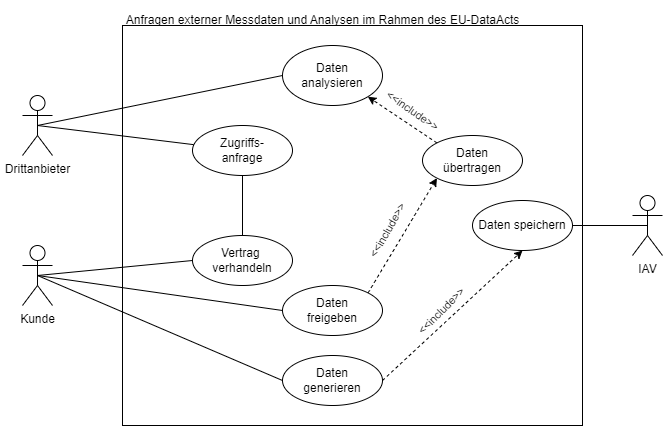
\includegraphics[scale=.6]{media/UseCase2}
    \caption{Use Case 1}
    \label{fig:UseCase2}
\end{figure}
\newpage
\section{Anfragen externer Messdaten und Analysen im Rahmen des EU-DataActs}
  Dieser Use Case beschreibt die Möglichkeit, dass ein Drittanbieter Zugriff auf die Betriebsdaten eines Fahrzeugs erhält, das von einem Kunden betrieben oder getestet wird. Dies geschieht im Rahmen des EU-DataActs, der den Austausch und die Bereitstellung von Daten zwischen Unternehmen fördert. Der EU Data Act spielt dabei eine entscheidende Rolle, da er sicherstellt, dass der Kunde das alleinige Recht über die Nutzung und Weitergabe der generierten Fahrzeugdaten besitzt.  \cite{bmdv2024} Dies bedeutet, dass der Kunde entscheiden kann, ob und in welchem Umfang er diese Daten an externe Dienstleister weitergeben möchte.
  \newline
  Der Prozess beginnt mit der kontinuierlichen Generierung von Betriebsdaten durch das Fahrzeug. Diese Daten umfassen verschiedene Aspekte des Fahrzeugbetriebs, wie Leistungskennzahlen, Kraftstoffverbrauch, Abnutzung und weitere für den Drittanbieter relevante Informationen. Die erfassten Daten werden in der IAV-internen Merida-Infrastruktur gespeichert und verwaltet, sodass sie jederzeit abrufbereit sind.
  \newline
  Wenn ein Drittanbieter Interesse an diesen Daten hat, stellt er eine offizielle Anfrage an den Kunden. Diese Anfrage betrifft spezifische Betriebsdaten, die für die Weiterentwicklung von Dienstleistungen oder Analysen des Drittanbieters von Nutzen sein könnten. Hier tritt der EU Data Act in Kraft, indem er sicherstellt, dass der Kunde in der Position ist, vollständig über die Verwendung seiner Daten zu entscheiden. Das gibt dem Kunden die volle Kontrolle über den weiteren Prozess.
  \newline
  \newline
  Nach der Anfrage folgt in der Regel eine Phase der Vertragsverhandlung, in der der Kunde und der Drittanbieter die Bedingungen für den Datenzugriff klären. Dabei geht es unter anderem um Fragen wie die Art der Daten, die freigegeben werden sollen, die Dauer des Datenzugriffs und mögliche Vergütungsregelungen. Der EU Data Act sorgt dafür, dass diese Verhandlungen fair und transparent ablaufen, sodass der Kunde jederzeit die Entscheidungsgewalt behält.
  \newline
  Sobald die Vertragsbedingungen festgelegt sind, entscheidet der Kunde, welche spezifischen Daten an den Drittanbieter übermittelt werden. Der Drittanbieter hat dann die Möglichkeit über das IAV Merida Request-Tool die gespeicherte Daten oder Analysen anzufragen. Es wird sichergestellt, dass diese Freigabe unter Berücksichtigung der Datenschutzbestimmungen erfolgt und dass nur die vereinbarten Daten bereitgestellt werden.
  \newline
  Nachdem die Daten oder Analysen an den Drittanbieter übermittelt wurden, kann dieser mit der Nutzung beginnen. Die gewonnenen Erkenntnisse könnten beispielsweise in die Entwicklung neuer Produkte oder Dienstleistungen einfließen, wobei der gesamte Prozess durch die klare Regelung des EU Data Acts strukturiert und kontrolliert wird.
  \newline
  Das folgende Diagramm bildet den beschriebenen Use Case ab und veranschaulicht die Interaktionen innerhalb des Prozesses von der Datengenerierung bis zur Speicherung. Zudem werden die Abhängigkeiten zwischen diesen Schritten deutlich gemacht.
  \begin{figure}[H]
      \centering
      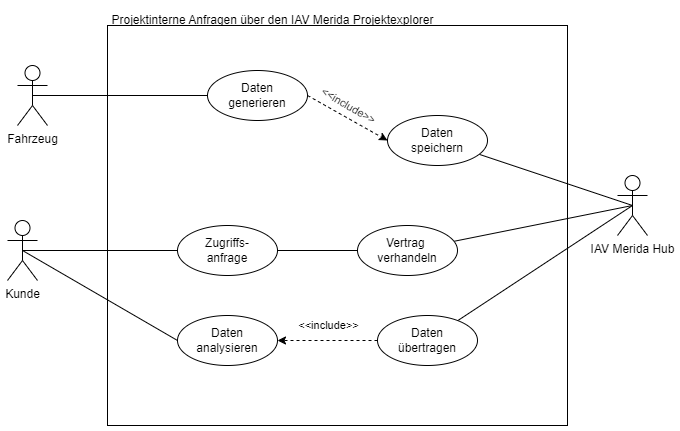
\includegraphics[scale=.6]{media/UseCase1}
      \caption{Use Case 2}
      \label{fig:UseCase1}
  \end{figure}
\newpage
\section{Anfragen von Daten eines Dritten und Bezahlung über Mobilfunkbetreiber}
Der folgende Use Case beschreibt einen Prozess, bei dem Fahrzeugführer ihre Betriebsdaten monetarisieren können, indem sie diese an interessierte Parteien wie zum Beipiel Versicherungsunternehmen oder OEMs verkaufen. Die dabei verwendeten Daten können von großem Nutzen für Unternehmen sein, die wertvolle Einblicke in die Fahrzeugnutzung gewinnen wollen, um ihre eigenen Produkte oder Dienstleistungen zu optimieren. Gleichzeitig ermöglicht dieser Prozess dem Fahrzeugführer, von den generierten Daten finanziell zu profitieren.
\newline
Auch hier werden die Fahrzeugdaten kontinuierlich erfasst und im Merida Hub gespeichert. Beispielsweise können dann Versicherungsunternehmen oder OEMs, die an diesen Daten interessiert sind, eine Anfrage an den Fahrzeugführer über einen Daten-Sammel- und Verteilungsdienst stellen, der die gesamte Abwicklung steuert. Diese interessierten Parteien sind insbesondere an den Nutzungsdaten des Fahrzeugs interessiert, um bessere Risikoanalysen durchzuführen oder spezifische Produkte für bestimmte Fahrzeugtypen zu entwickeln.
\newline
\newline
Nach der Anfrage folgt eine Phase der Vertragsverhandlung, in der die Bedingungen für den Datenzugriff geklärt werden. Der Fahrzeugführer, der als Datenverkäufer agiert, hat dabei die Möglichkeit, die Konditionen auszuhandeln und den Preis für die Bereitstellung seiner Daten festzulegen. Ziel ist es, eine faire und ausgewogene Vereinbarung zu treffen, die sowohl den Interessen des Fahrzeugführers als auch denen der interessierten Parteien gerecht wird.
\newline
Die Datenübertragung erfolgt sicher und kontrolliert über das 5G-Netzwerk eines Netzbetreibers wie Telefónica. Dieser Mobilfunkbetreiber spielt eine zentrale Rolle, indem er nicht nur die Datenübertragung gewährleistet, sondern auch die Zahlungstransaktionen abwickelt. Dies sorgt für eine reibungslose und schnelle Bereitstellung der Daten sowie eine unkomplizierte Bezahlung des Fahrzeugführers.
\newline
Die interessierten Parteien nutzen die erhaltenen Daten anschließend, um ihre Produkte und Dienstleistungen zu verbessern. Beispielsweise könnten Versicherungsunternehmen anhand der Fahrzeugnutzungsdaten maßgeschneiderte Versicherungspakete anbieten, die auf das individuelle Fahrverhalten des Fahrzeugführers zugeschnitten sind. OEMs hingegen könnten die Daten verwenden, um die Leistung ihrer Fahrzeuge besser zu verstehen und zukünftige Modelle zu optimieren.
\newline
Dieser Use Case bietet somit allen beteiligten Akteuren Vorteile: Der Fahrzeugführer profitiert finanziell von seinen Daten, während die interessierten Unternehmen wertvolle Einblicke gewinnen, um ihre Geschäftsprozesse und Angebote zu verbessern.
\newline
Das nachstehende Diagramm veranschaulicht den Use Case für die Anfrage von Daten eines Dritten sowie die Bezahlung über einen Mobilfunkanbieter.
\begin{figure}[H]
    \centering
    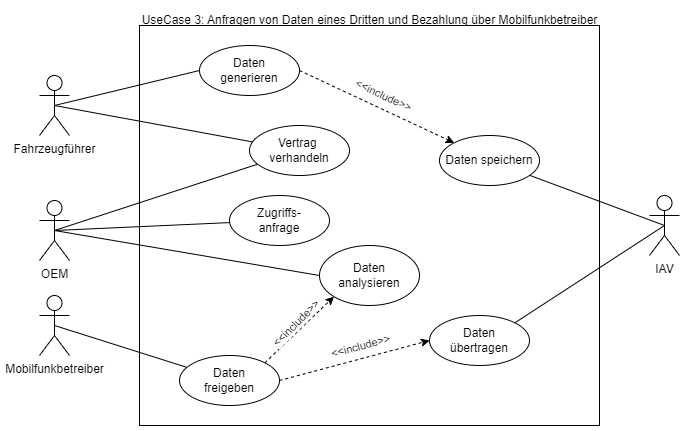
\includegraphics[scale=.6]{media/UseCase3}
    \caption{Use Case 3}
    \label{fig:UseCase3}
  \end{figure}
\label{chap:kapitel4}
